\chapter{Présentation de la problématique (sujet du stage)}
\minitoc
    \section{Présentation du sujet}
    Projet avec le laboratoire de \textit{Biologie} de l'\textit{Université des Antilles}, le projet concerne en l'analyse de déplacement de Gerridés afin de déterminer leur préférence sur des zones marquées par des odeurs, en environnement contrôlé.

    \section{Objectifs}
    Ma mission est de réalisé l'installation et de configurer un dispositif de capture vidéo réalisé par un \textit{Raspberry Pi} ainsi que de développer une application conviviale pour la gestion des vidéos.

    \section{Présentation des outils}
        \subsection{Raspberry Pi}
        Le \textit{Raspberry Pi} est un ordinateur portable de petite taille, doté d'un processeur ARM et d'un système d'exploitation Linux.
        \begin{center}
            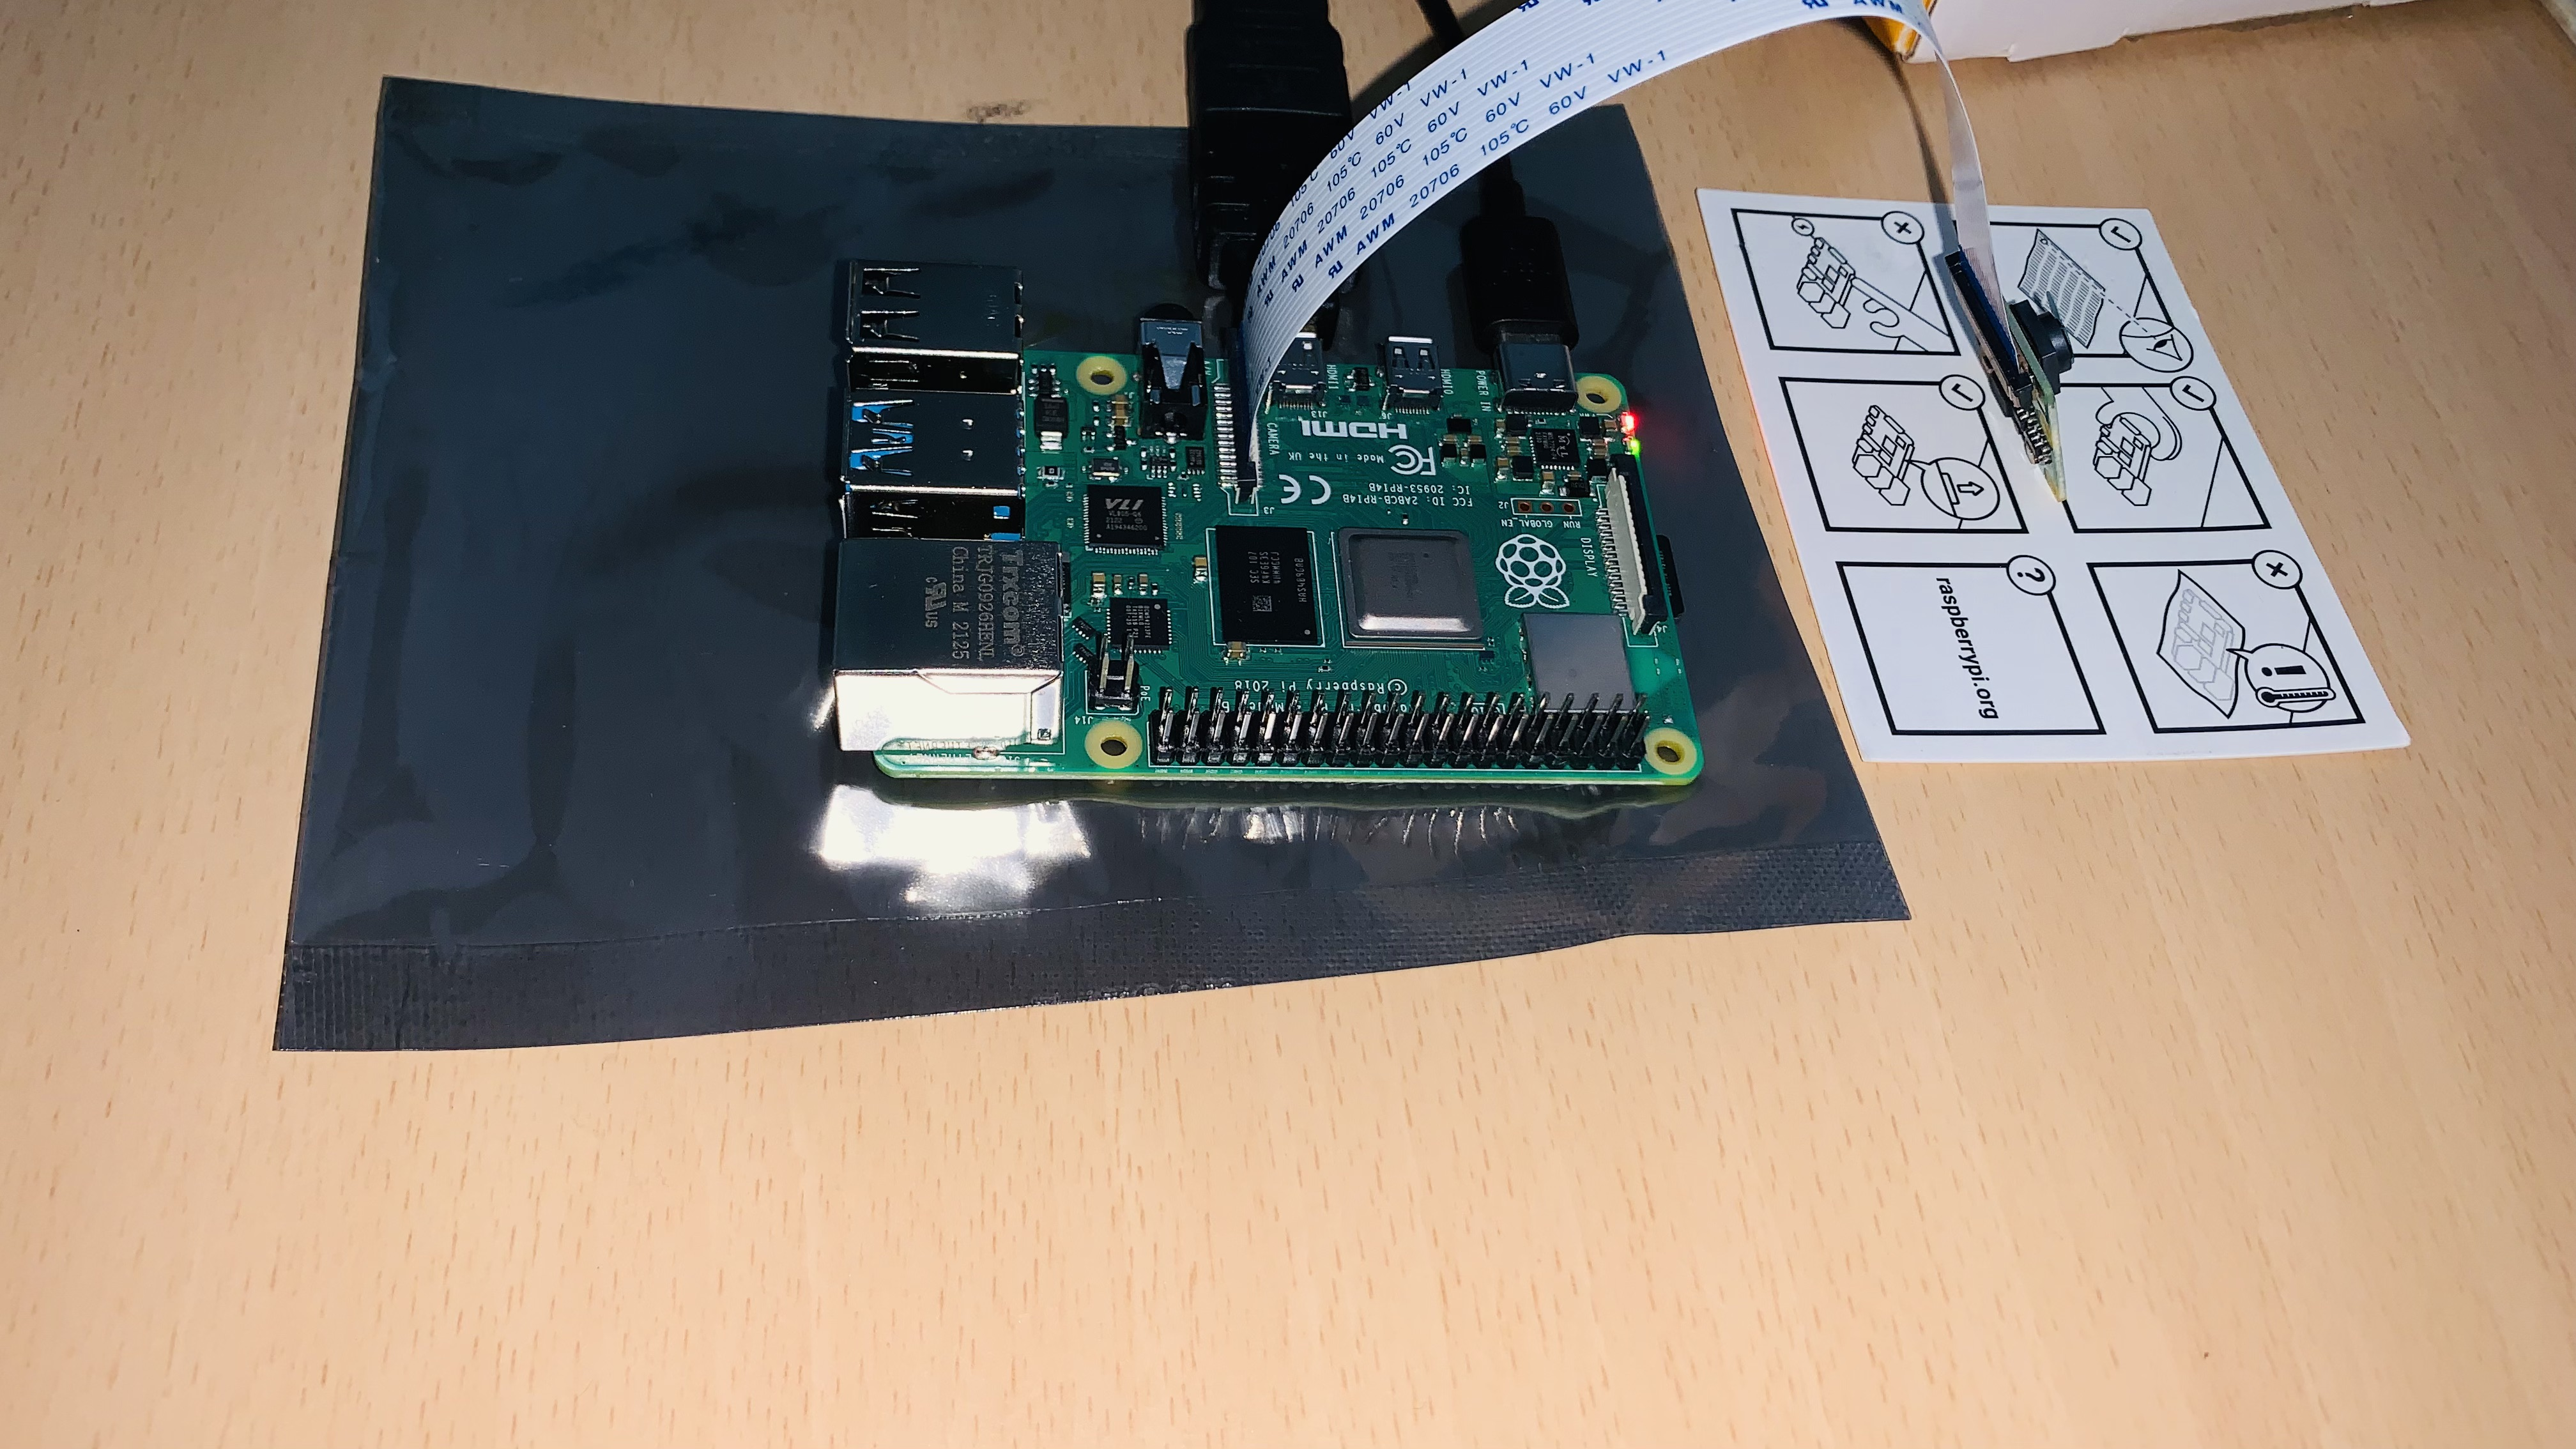
\includegraphics[scale=0.05]{raspberry_pi.jpeg}
        \end{center}
        \subsection{Module de capture vidéo (Raspberry Pi) V2}
        Le module de capture vidéo (Raspberry Pi) V2 est un module de captation vidéo qui permet de capturer des images et des vidéos.
        \begin{center}
            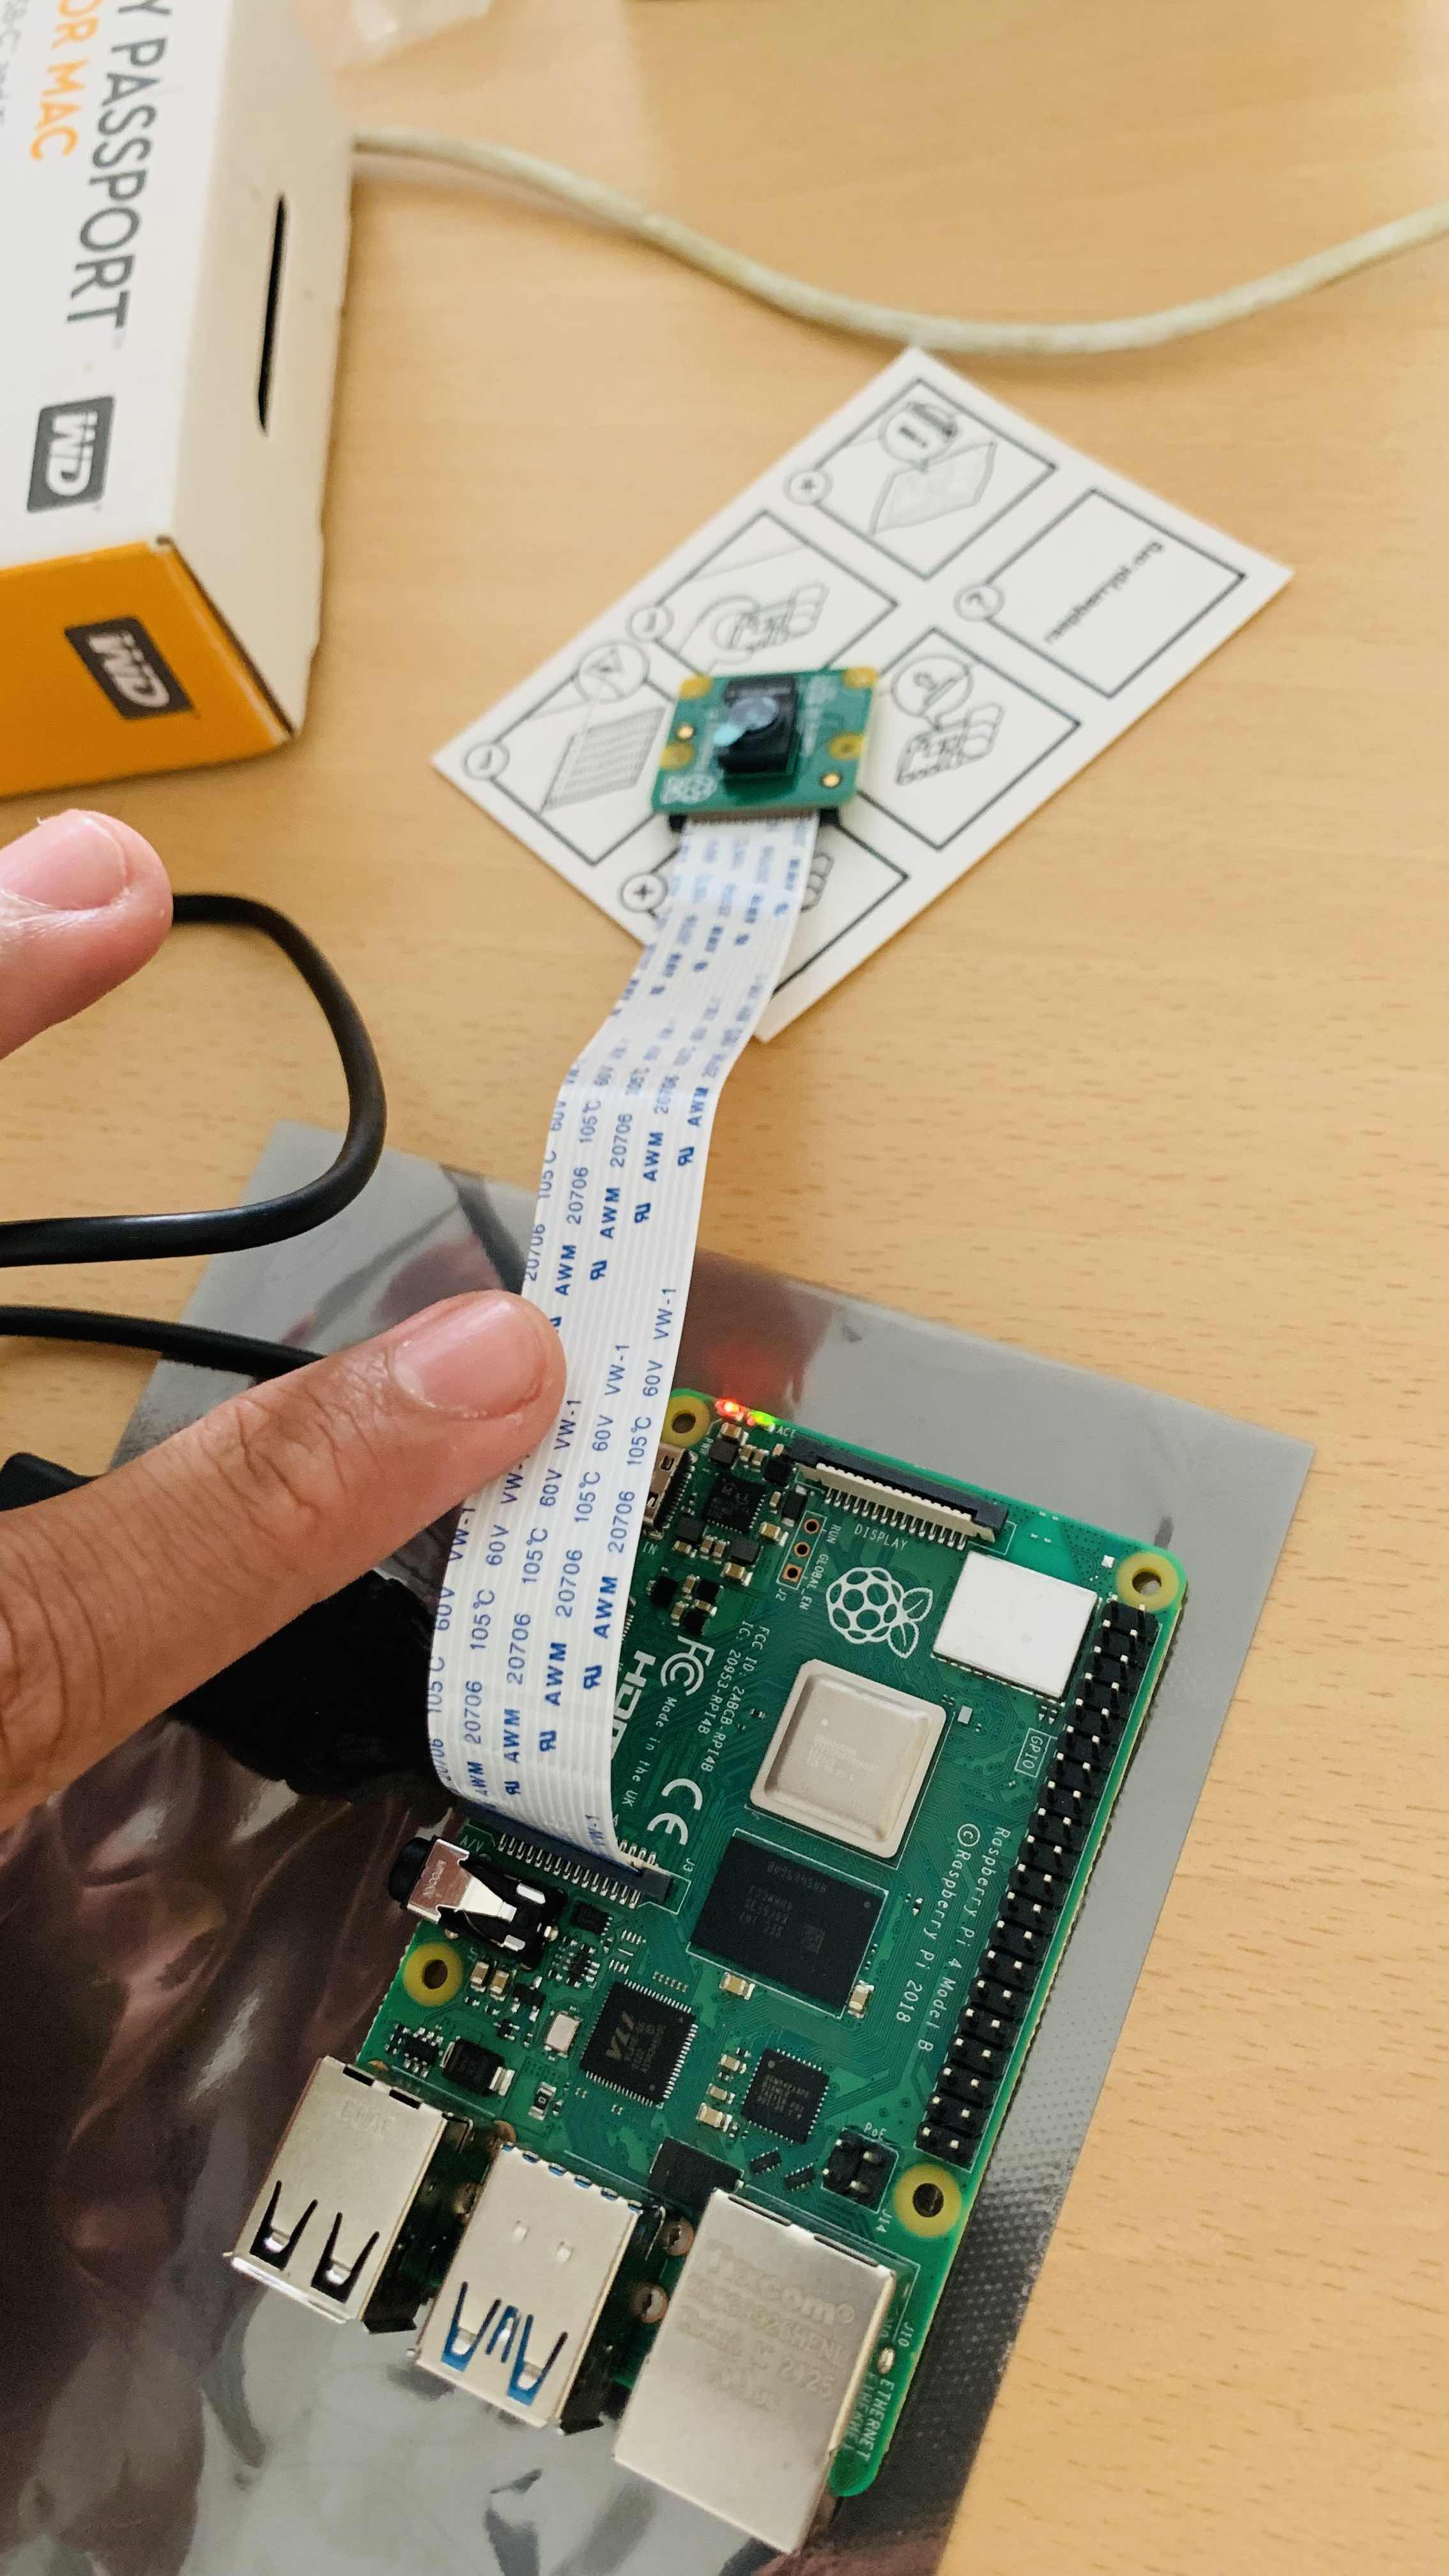
\includegraphics[scale=0.05]{module_camera_v2.jpeg}
        \end{center}

        % \vspace{5cm}
        
        \subsection{Ecran LCD (Raspberry Pi) tailles}
        Le \textit{Raspberry Pi} est doté d'un écran LCD de 7 pouces qui permet de visualiser les images et les vidéos et d'interagir avec l'ordinateur grâce à son tactile. 
        \begin{center}
            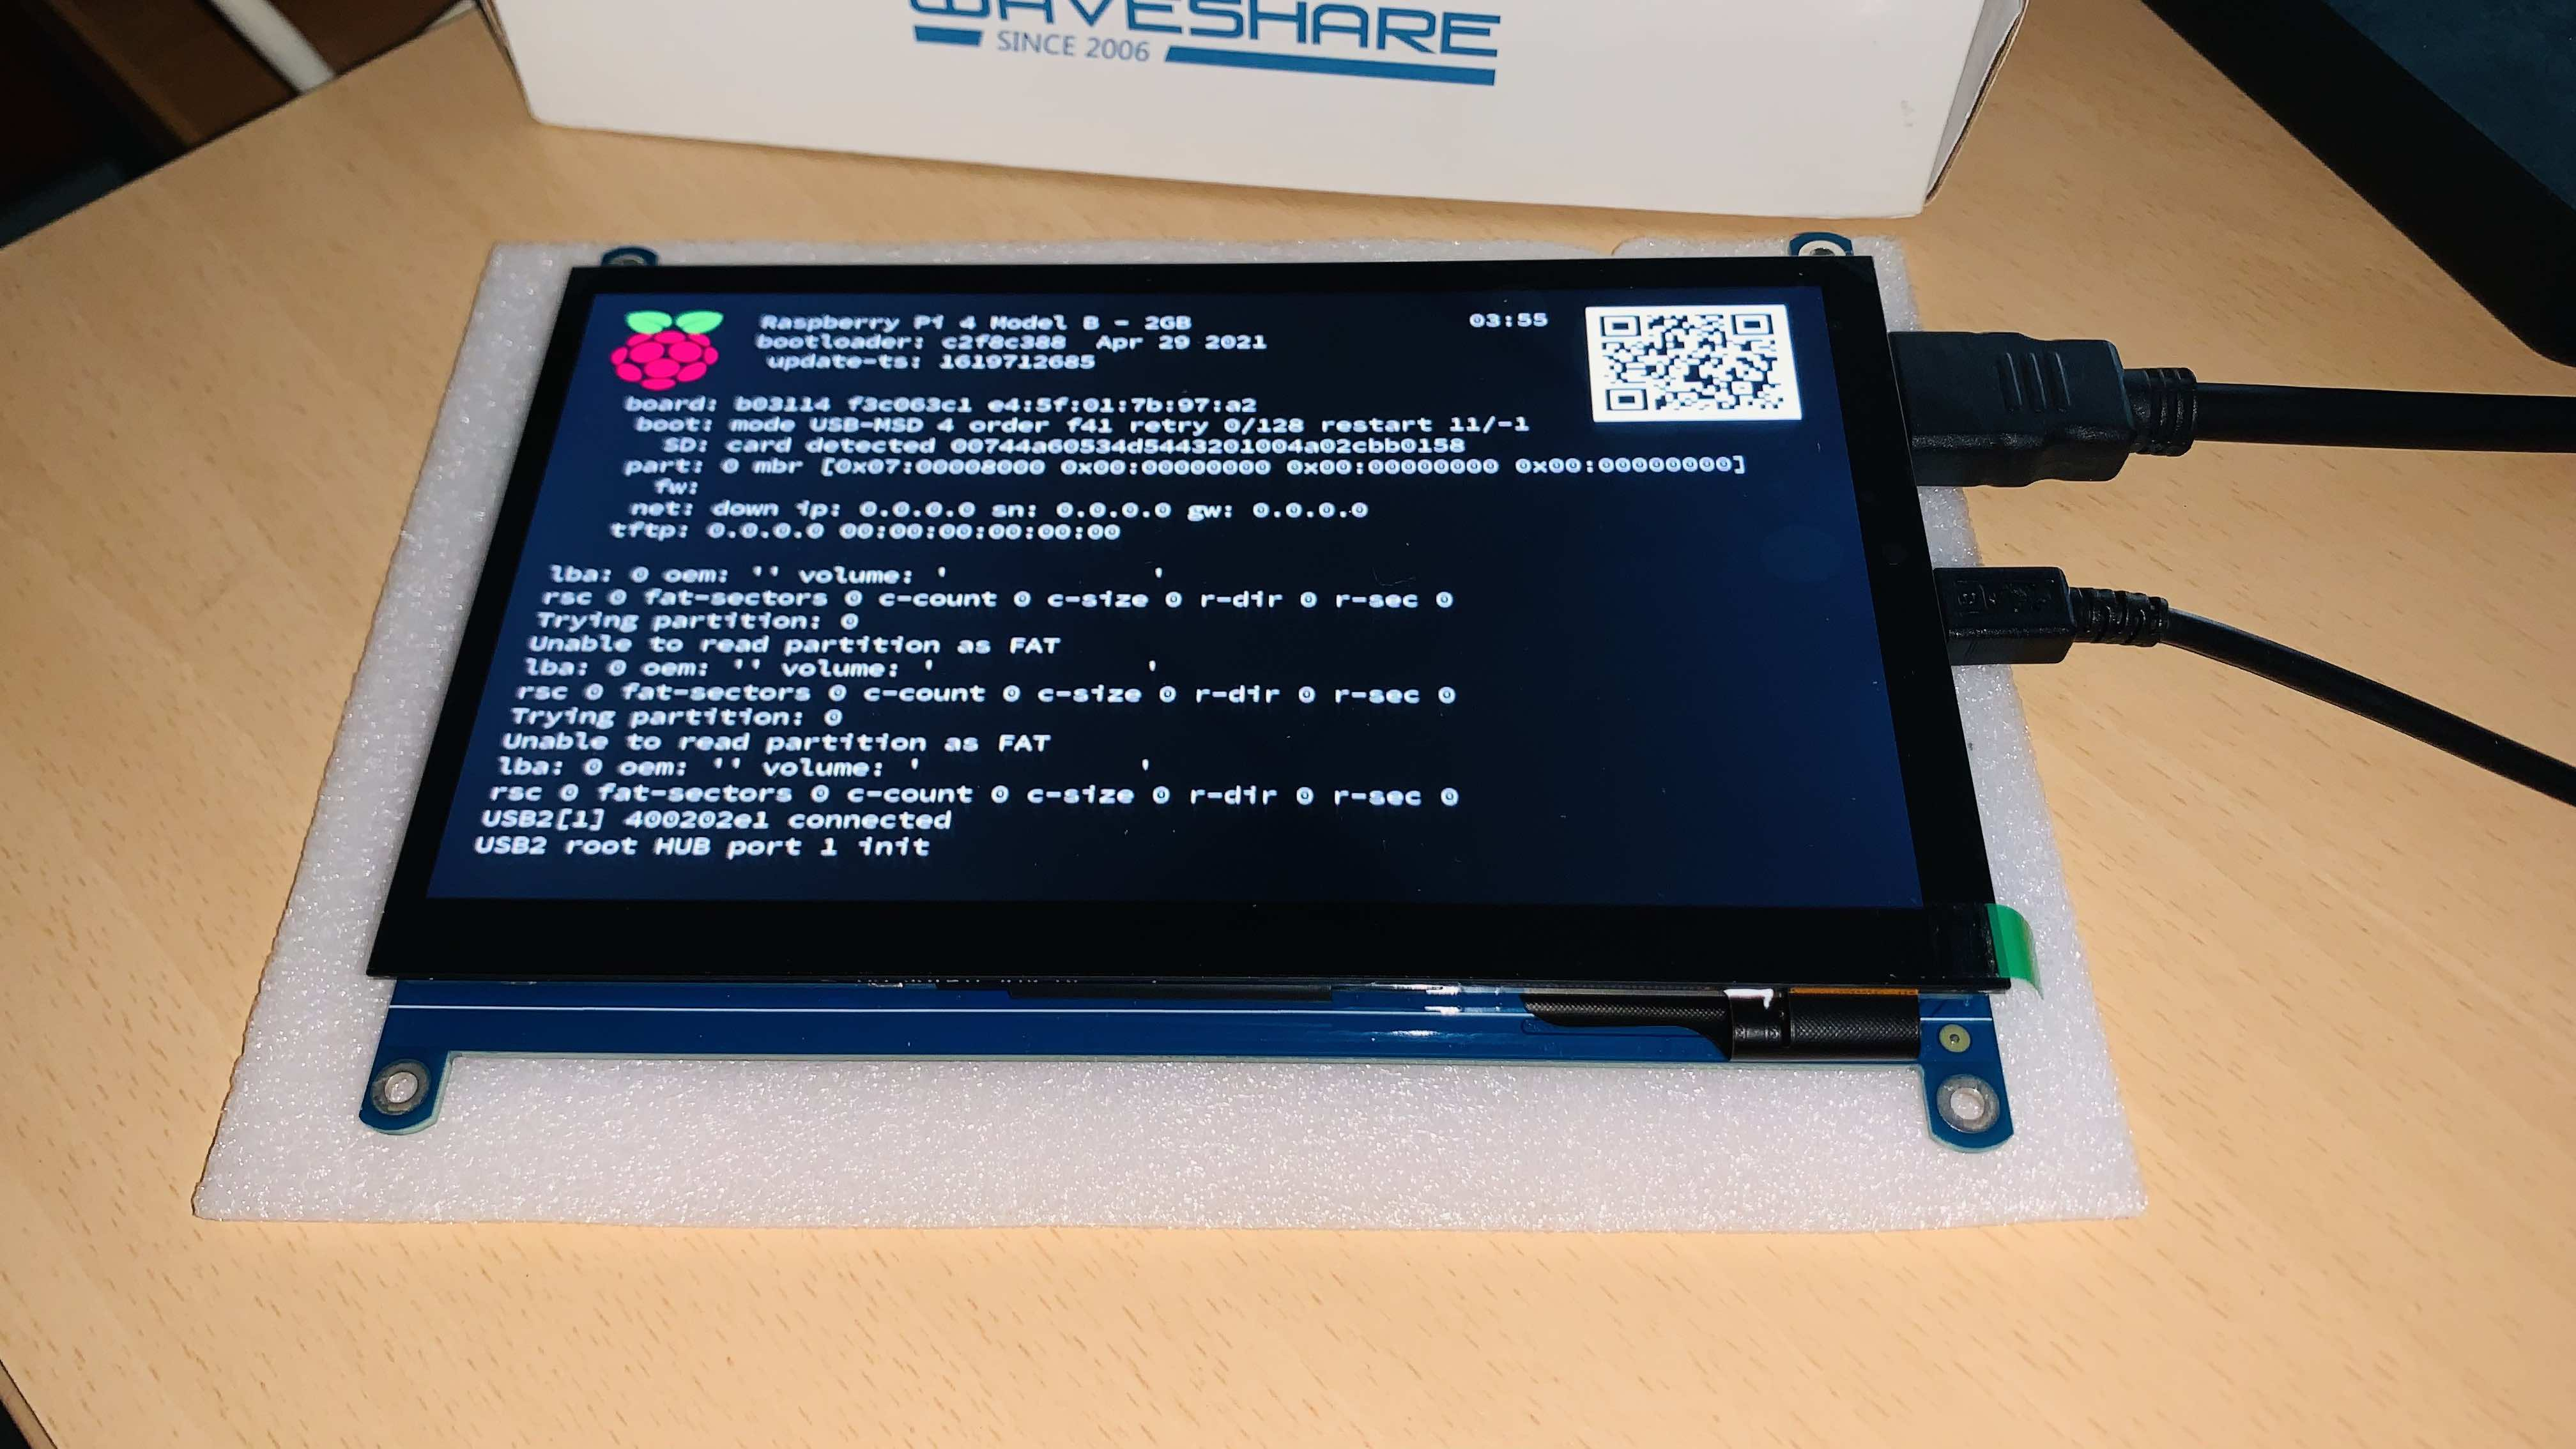
\includegraphics[scale=0.05]{raspberry_pi_lcd.jpeg}
        \end{center}

    \section{Description, résultats attendus et objectifs}
    \section{Etude du besoin}
        \subsection{Contexte}
        \subsection{Analyse du besoin}
        \subsection{Définition des besoins}
        
    \section{Choix des technologies}
        \subsection{Choix du langage Python}
        \subsection{Choix l'API PiCamera}
        \subsection{Choix de la bibliothèque Tkinter}
        \section{Projet : Montage du dispositif de capture vidéo}
      
        \subsection{Objectifs}
            \begin{itemize}
                \item Montage du dispositif de capture vidéo
                \item Acquisition des données
                \item Traitement des données
                \item Visualisation des données
            \end{itemize}
    

    \section{Projet : Rélisation du logiciel de capture vidéo}
        \subsection{Objectifs}
            \begin{itemize}
                \item Réalisation du logiciel de capture vidéo
                \item Acquisition des données
                \item Traitement des données
                \item Visualisation des données
            \end{itemize}